\documentclass[reprint,nofootinbib,...]{revtex4-1} 
%\documentclass[draft,nofootinbib,...]{revtex4-1} 
\usepackage{amsmath}%
\usepackage{amsthm,amssymb}
\usepackage{graphicx}
\usepackage{epstopdf}
\usepackage{xcolor}
\usepackage{algcompatible}
\usepackage[size=small]{caption}
\usepackage{etoolbox}
\usepackage{booktabs}
\usepackage{multirow}
\usepackage[utf8]{inputenc}
\usepackage[colorinlistoftodos]{todonotes}

\usepackage[hyperfootnotes=true]{hyperref}
\hypersetup{
 colorlinks=true,
 citecolor=blue,
 linkcolor=blue,
 urlcolor=blue}

%%% ----------------------------------------------------------------------
\begin{document}

%Title of paper
\title{AI Safety for High Energy Physics}

\author{Benjamin Nachman}
\email{bpnachman@lbl.gov}

\affiliation{Physics Division, Lawrence Berkeley National Laboratory, Berkeley, CA 94720, USA}

\author{Chase Shimmin}
\email{chase.shimmin@yale.edu}

\affiliation{Department of Physics, Yale University, New Haven, CT 06511, USA}

\begin{abstract}
Since the first application of deep learning on `low-level' features for classification in high-energy physics (HEP)~\cite{Baldi:2014kfa}, there has been a rapidly expanding literature on the adaptation of industrial deep learning techniques as well as the development of novel methods.  The overall conclusion from this impressive and extensive set of studies is that rarer and more complex signatures can be identified with the new set of powerful tools from deep learning.  However, there is an unstudied risk associated with combining the traditional HEP workflow and deep learning with high-dimensional data.  In particular, calibrating and validating deep networks in their natural high dimensionality is not possible and therefore current methods may be biased in ways that are not covered by current uncertainty estimates.  By borrowing ideas from AI safety, we illustrate these potential issues and propose a method to bound the size of unaccounted for uncertainty.  In addition to providing a pragmatic diagnostic, hopefully this work will begin a dialogue within the community about the robust application of deep learning to new particle searches.
\end{abstract}

\date{\today}
\maketitle

%%%%%%%%%%%%%%%%%%%%%%%%%%%%%

In collider-based high-energy physics (HEP), simulations modeling length scales from sub-nuclear reactions all the way to macroscopic detector-length scales are critical for scientific inference by connecting fundamental theories to observable quantities.  These simulations are excellent, but are an approximation to nature and therefore must be calibrated with data. In the quest for new particles, calibrated simulations of the Standard Model (SM) are compared with data to search for potential anomalies.

In the traditional paradigm, a discriminating observable $m$ is used to isolate a region of phase space $m<c$ where contributions from new particles are expected to be small compared with the SM background processes.  In this \textit{control region}, the predicted cross-section is scaled to match the data and then the scaled differential cross-section from simulation is used to estimate the Standard Model contribution in a \text{signal region} with $m\gg c$.  Theoretical uncertainties on the extrapolation are estimated by repeating this procedure with a variety of simulations.

Deep learning offers a new set of tools in HEP for seeking out new particles using high-dimensional, low-level information~\cite{Baldi:2014kfa,Larkoski:2017jix,Radovic:2018dip,Guest:2018yhq}. A growing number of searches at the Large Hadron Collider are using deep learning methods to construct $m$. The control region method is the baseline approach for estimating the SM background in the nascent deep learning era.

A potential problem of the control region method with deep learning is that the calibration procedure may not sufficiently probe the high dimensionality of the feature space.  For example, if $\mathcal{O}(1000)$ dimensions are used for training a neural network, but only $\mathcal{O}(1)$ simulation variations are considered for the uncertainty on the calibration (as is common), then the prediction in the signal region may be incorrect: the uncertainty may be much smaller than the potential bias.

This work uses methods from AI safety to diagnose the sensitivity of the current methodology to under-constrained phase spaces.  In particular, a standard high-dimensional classification problem is used to illustrate the sensitivity to small perturbations in measured particle properties and also to devise a sensitivity diagnostic with a directed adversarial attack.  Certainly nature is not evil, but without any good estimate of high dimensional correlated uncertainty, this bound can be used to demonstrate robustness. 

As one of the first examples of high-dimensional deep learning in high-energy physics, jet classification~\cite{Larkoski:2017jix} is used as the prototypical example.  Jets are collimated sprays of particles resulting from high energy quark and gluon fragmentation.  As such, one can represent a jet $J_i$ by its constituent particle momenta $\{(p_{T,ij},\eta_{ij},\phi_{ij})\}\in\mathbb{R}^{3N}$, ignoring particle masses and other quantum numbers.  The dataset simulated~\cite{gregor_kasieczka_2019_2629073} includes generic quark and gluon scattering as the background process and boosted new particles decaying into jets as the signal process. Pythia~8~\cite{Sjostrand:2006za,Sjostrand:2007gs} and Delphes 3.4.1~\cite{deFavereau:2013fsa} are used to simulate the scattering process and detector response, respectively.  Jets are clustered using Fastjet~\cite{Cacciari:2011ma,Cacciari:2005hq} vis pyjet~\cite{noel_dawe_2019_2672944} implementing the anti-$k_t$ algorithm with radius parameter $R=1$~\cite{Cacciari:2008gp}.

To demonstrate the sensitivity of existing methods to small perturbations to the input particles in high dimensions, a fast gradient sign method (FGSM) is deployed~\cite{DBLP:journals/corr/GoodfellowSS14}.  The idea is that individual jets are perturbed $J\mapsto \delta J_i$ based on the gradient of the classification loss.  Each jet is independently modified, which is an unlikely scenario for high-dimensional mis-modeling, but is a robust indication of a classifier's sensitivity to fixed small perturbations.  A universal modifier is discussed later.  A deep neural network $f(J_i)\mapsto [0,1]$ is trained in the usual way $f=\text{argmin}_{f'}\mathcal{L}(F'(J),y)$, $y\in\{0,1\}$, where $\mathcal{L}$ is the loss function (in this case, cross-entropy).  Networks are trained with Keras~\cite{keras} using the Tensorflow~\cite{tensorflow} backend and optimized using Adam~\cite{adam}.  To compare the sensitivity of a deep neural network trained directly on the natural high-dimensionality with traditional methods, a second network is trained whose first layer is a ratio of energy correlation functions~\cite{Larkoski:2013eya} known as $D_2$~\cite{Larkoski:2014gra}.

The FGSM modification is then given by

\begin{align}
\label{eq:FGSM}
f(J_i+\epsilon\times\text{sign}(\Delta_J(\mathcal{L}(f,J))|_{J=J_i}),
\end{align}

\noindent where $\epsilon=(\epsilon_{p_T},\epsilon_\eta,\epsilon_\phi)^N, \epsilon_i\ll1$ is a small perturbation.  In the example below, $\epsilon=(2,20,20)\times 10^{-4}$.  The process illustrated in Eq.~\ref{eq:FGSM} is repeated $N=10$ times.  Figure~\ref{fig:FGSM} blah...

\begin{figure}[h!]
\centering
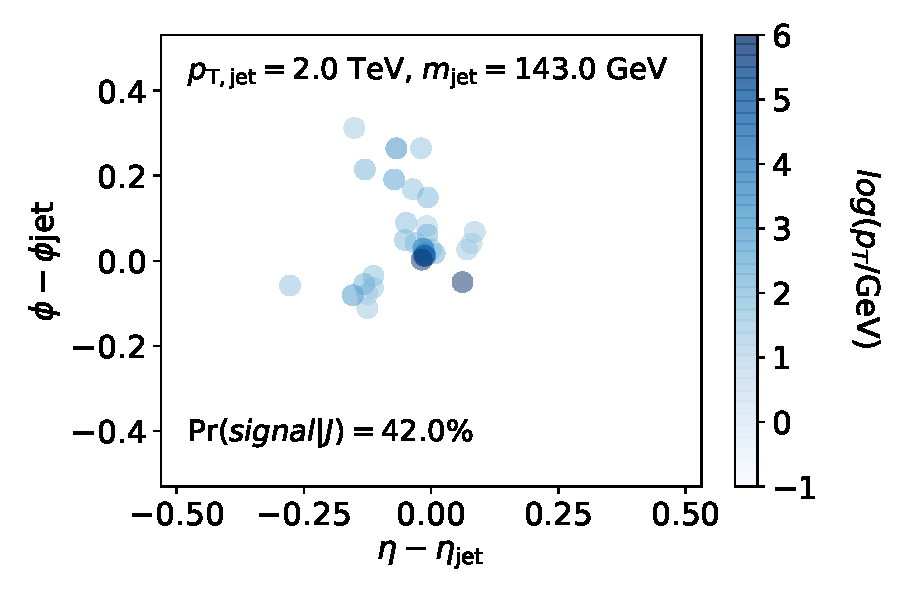
\includegraphics[width=0.15\textwidth]{figures/panel_1.pdf}
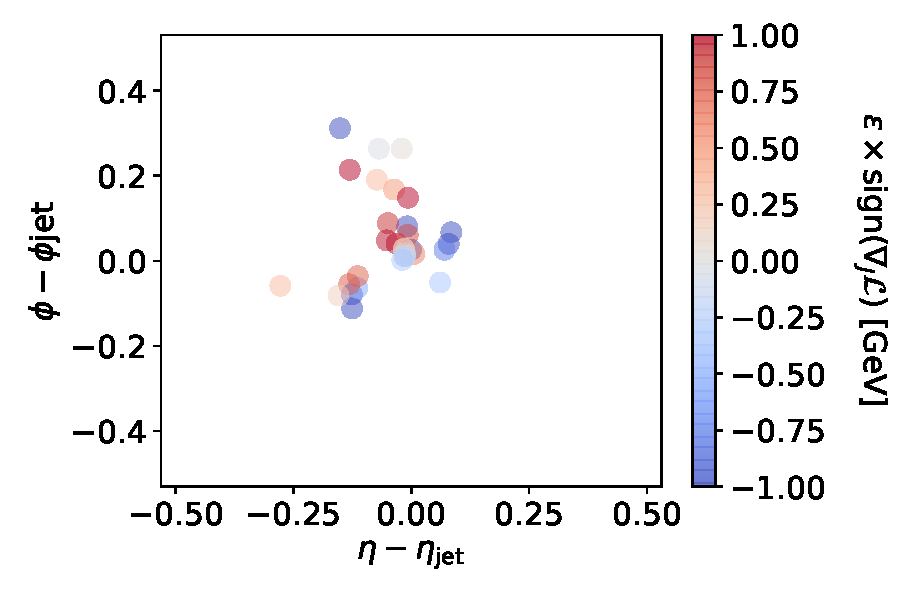
\includegraphics[width=0.15\textwidth]{figures/panel_3.pdf}
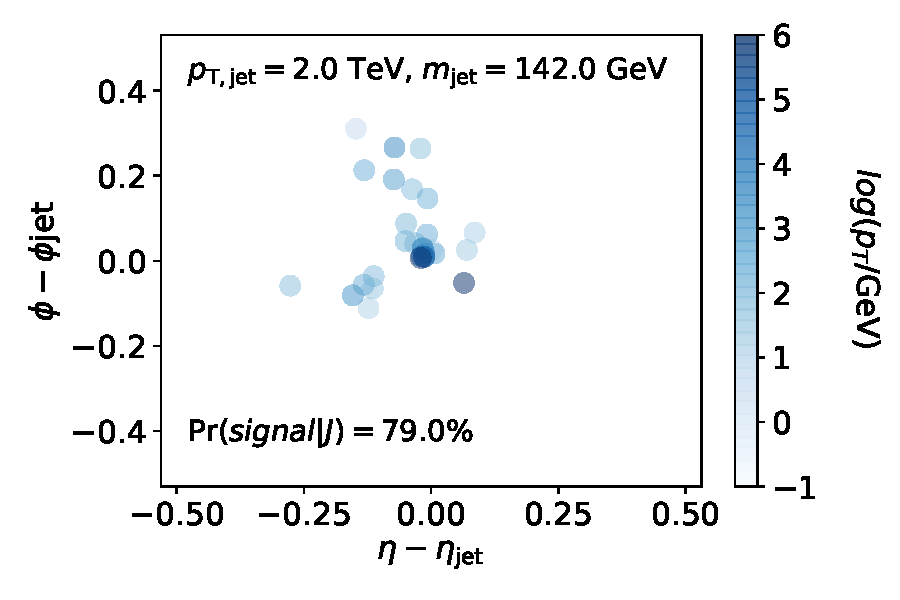
\includegraphics[width=0.15\textwidth]{figures/panel_2.pdf}
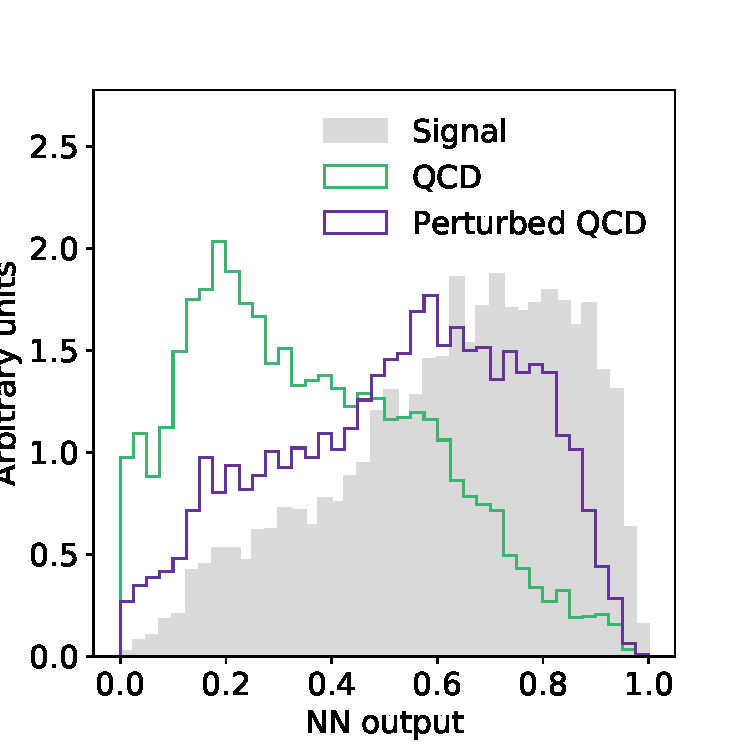
\includegraphics[width=0.23\textwidth]{figures/NN_FGSM.pdf}
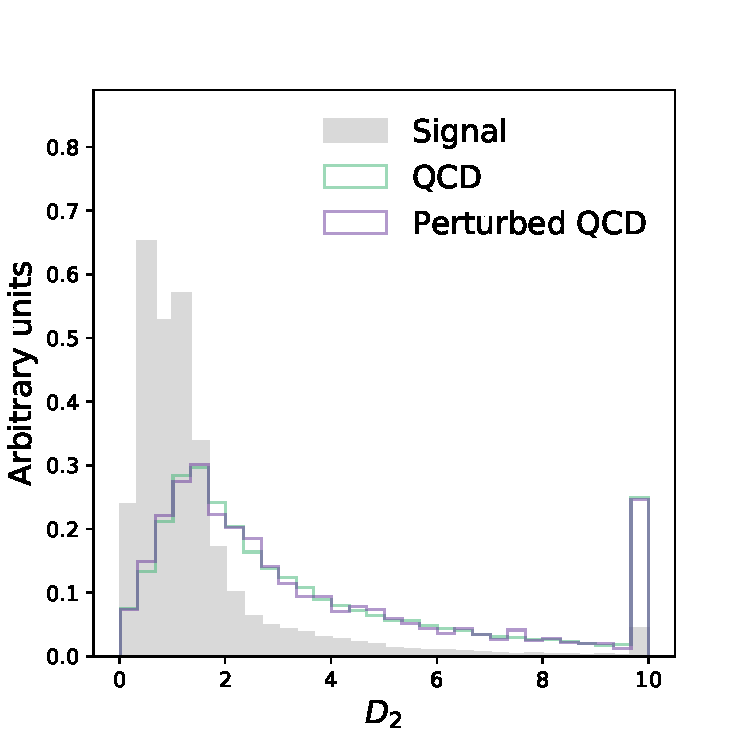
\includegraphics[width=0.23\textwidth]{figures/D2_FGSM.pdf}
\caption{The application of FGSM to jets.  The top row of plots show image representations of a single jet before (left) and after (right) an FGSM perturbation.  The grayscale indicates the particle $p_T$.  The middle plot illustrates the difference between the plots.  The lower plots show NN (left) and $D_2$ histograms for signal and background before and after the FGSM perturbation.  Both sets of jets are perturbed by the same amount, yet the distribution of $D_2$ is largely unchanged. }
\label{fig:FGSM}
\end{figure}

While the FGSM illustrated the sensitivity to small perturbations for single jets, it does not show how systematic ensemble perturbations could modify the classifier performance.  Blah...

\begin{align}
\label{eq:global}
g=\text{argmin}_{g'}\left[\mathcal{L}_\text{xe}(f(J+\delta J),\bar{y})+\mathcal{L}_\text{jet}(J,J+\Delta J)\right],
\end{align}

Conclusions and outlook...

\section*{ACKNOWLEDGMENTS}

This work is supported by the DOE under contract DE-AC02-05CH11231. 

\bibliography{myrefs}

\end{document}